\documentclass[12pt]{article}
\usepackage[a4paper, margin=.30in]{geometry}
\usepackage{graphicx ,
            wrapfig,
            xcolor, 
            enumerate,
            amsmath,fontenc, mhchem  ,tcolorbox, chemfig, makecell
            }
\usepackage{multirow}
\newcommand\headerMe[2]{\noindent{}#1\hfill#2}
\renewcommand{\thesection}{\Roman{section}}

\author{Zakaria HAOUZAN}
\date{\today}

\begin{document}
% headers --------------
\headerMe{Matière : Physique-Chimie}{Professeur : Zakaria HAOUZAN}\\
\headerMe{Unité : Méthode de
contrôle de
l’évolution des
systèmes
chimiques }{Établissement : Lycée SKHOR qualifiant}\\
\headerMe{Niveau : 2BAC-SM-X}{Heure : 12H}\\

% ------Content ________
\begin{center}

  \Large{Leçon $N^{\circ} 12 $: \color{red} Contrôle de l’évolution de systèmes chimiques}
\end{center}

%\begin{wrapfigure}[10]{r}{0.5\textwidth}
%    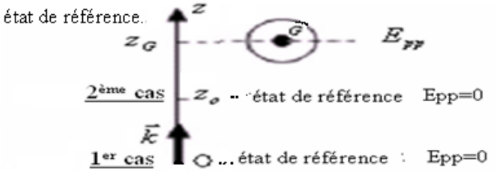
\includegraphics[width=0.5\textwidth]{./img/img00.png}
%\end{wrapfigure}


%\begin{tcolorbox}[colback=pink!10!white,
                  %colframe=blue!15!gray,
                  %title=Application -1- :
                 %]


  %\begin{wrapfigure}[10]{r}{0.3\textwidth}
  %\vspace{-2cm}
    %\includegraphics[width=0.3\textwidth]{./img/Mode_opératoire_dosage:.png}
%\end{wrapfigure}

\section{L'estérification rapide : préparation d'un ester }
\subsection{Estérification rapide:}
La synthèse des esters à partir des acides carboxyliques est une réaction lente et limitée, elle devient plus rapide et
totale lorsque l’acide carboxylique est remplacé par son anhydride.

anhydride d'acide + alcool $\rightarrow$ Ester + acide


$$\chemfig{R-C(=[::+60]O)-[::-10]O-[::-120]C(=[::+60]O)-[::-50]R} + R'-OH \rightarrow \chemfig{R-C(=[6]O)-O-R'} + \chemfig{R-C(=[::+60]O)(-[::-60]OH)}$$

Cette réaction est rapide et totale (On l’appelle estérification rapide avec l’anhydride de l’acide carboxylique )

Exemple : synthèse de l'aspirine 

L'aspirine (ou acide acétylsalicylique) est un ester synthétisé à partir de l'acide salicylique et de l'anhydride éthanoïque.

$$\chemfig{*6(-=(-OH^{-})-(-COOH)=()-=)} + \chemfig{CH_3-C(=[6]O)-O-C(=[6]O)-CH_3} \rightarrow  \chemfig{*6(-=(-O(-[::+30]C(=[6]O)-CH_3))-(-COOH)=()-=)} + CH_3COOH$$

acide salicylique + anhydride éthanoïque $\rightarrow $ aspirine + acide acétique


\textbf{Autre exemple: synthèse de l'éthanoate de 3-méthylbutyle.}

$\chemfig{CH_3-C(=[6]O)-O-C(=[6]O)-CH_3} + \chemfig{CH_3-CH(-[2]CH_3)-CH_2-CH_2-OH}$ 

$\rightarrow$ 

$\chemfig{CH_3-C(=[::60]O)(-[::-60]O-CH_2-CH_2-CH(-[2]CH_3)-CH_3)} + \chemfig{CH_3-C(=[::+60]O)(-[::-60]OH)}$


\section{Réaction de saponification : }
\subsection{Définition}

Les bases fortes comme l'hydroxyde de sodium (ou la potasse) réagissent avec les esters selon une réaction totale appelée :
réaction de saponification. 

$$RCOOR' + (Na^+ + OH^-) \rightarrow (RCOO^- + Na^+) + R'OH$$

ester + soude $\rightarrow$ carboxylate de sodium (savon) + alcool 


Pour préparer le savon on mélange de l’huile et de soude mis en solution dans l'éthanol et on ajoute la pierre ponce au
mélange (pour régulariser l'ébullition) puis on chauffe à reflux, vers 120 °C pendant une demi-heure.


\begin{center}
	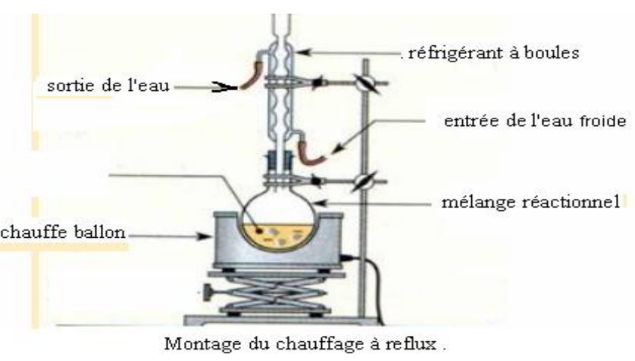
\includegraphics[width=0.5\textwidth]{./img/reflux.png}
\end{center}


Le savon formé est séparé de l'alcool et de l’excès de soude par relargage dans une solution concentrée de chlorure de sodium
car le savon qui n'est trops soluble dans l’eau salée précipite ce qui permet de le recueillir par filtration.
. Le relargage est un procédé qui consiste, lorsqu'un produit est soluble à la fois dans l'eau et dans un autre liquide non
miscible à l'eau, à ajouter à ce mélange liquide un peu de chlorure de sodium pour faciliter la séparation.

\subsection{Application: saponification des acides gras.}
Les acides gras sont des acides carboxyliques RCOOH ayant des chaines carbonées longues .exemple : $C_{17}H_{35}COOH$.
La réaction d'un glycérol avec acide gras conduit à un triester.

La réaction d'un glycérol $\chemfig{CH_2(-[6]CH(-[6]CH_2-OH)-OH)-OH}$
 avec acide gras $R-COOH$ conduit à un  triester 

 $\chemfig{CH_2(-[6]CH(-[6]CH_2-O-C(=[::-60]O)-R)-O-C(=[::-60]O)-R)-O-C(=[::-60]O)-R}$

Le triester résultant est un corps gras, en le faisant réagir avec la soude on obtient du savon. 


 $\chemfig{CH_2(-[6]CH(-[6]CH_2-O-C(=[::-60]O)-R)-O-C(=[::-60]O)-R)-O-C(=[::-60]O)-R}$ + $3(Na^+ + OH^-)$ $\rightarrow$ $\chemfig{CH_2(-[6]CH(-[6]CH_2-OH)-OH)-OH} + 3RCOONa$


 triester +la soude $\rightarrow$ glycérol + le savon


 \subsection{Propriétés du savon:}
 Le savon est un mélange d'ions carboxylates $RCOO^-$ et d'ions sodium $Na^+$ (ou de potassium $K^+$ ) dont les radicaux $-R$ sont
dérivés d’acides gras à longues chaînes carbonées (plus de 10 atomes de carbone).

L'ion carboxylate $RCOO^-$ constituant le savon est une base qui appartient au couple acide/base $RCOOH/RCOO^-$ ,il
est constitué de deux parties:

\begin{itemize}

	\item Une tête soluble dans l’eau $-COO^-$ appelée la partie hydrophile.
	\item Une longue chaîne carbonée (la queue) , insoluble dans l'eau appelée la partie hydrophobe. Les parties hydrophobes
sont solubles dans les huiles et les graisses constituant la saleté du linge.
\item Ainsi les particules savonneuses peuvent s’enfoncer dans les tâches organiques et les retirer du tissu.
\end{itemize}


\begin{center}
	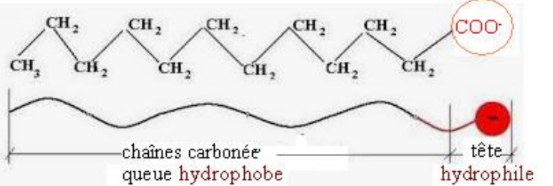
\includegraphics[width=0.5\textwidth]{./img/file.png}
\end{center}




. Les têtes hydrophiles sont attirées par l’eau, tandis que les queues hydrophobes restent à l’extérieur formant des bulles et de la
mousse.. Le savon est un bon nettoyant ayant la propriété principale est d’améliorer le pouvoir mouillant de l’eau.Les parties
hydrophobes sont solubles dans les huiles et les graisses constituant la saleté du linge.

\section{Contrôle de l'évolution d'un système chimique : }
\subsection{Rappel:} 

En remplaçant l'un des réactifs on peut contrôler l'évolution d'un système chimique et rendre une réaction limitée réaction totale (voir estérification avec un anhydride de l'acide carboxylique) et on peut aussi contrôler l'évolution d'un
système chimique en utilisant l'un des facteurs cinétique.


\subsection{Contrôle de l'évolution d'un système chimique par un catalyseur:}
Un catalyseur est une substance qui accélère une réaction chimique sans apparaître dans l’équation de la réaction.

\begin{itemize}
	\item Lorsque le catalyseur appartient à la même phase que les réactifs, la catalyse est dite \underline{homogène}.
	\item Lorsque le catalyseur n’appartient pas à la même phase que les réactifs, la catalyse est dite \underline{hétérogène}.
\item Lorsque le catalyseur est une enzyme, la catalyse est \underline{enzymatique}.
\item L'utilisation de certains catalyseurs sélectifs peut conduire à des produits différents.

\end{itemize}
Exemple : La vapeur d'éthanol à 300oC envoyée sur deux catalyseurs différents :

-Avec le catalyseur alumine $Al_2O_3$, on obtient de l'éthylène :$CH_3CH_2OH\rightarrow CH_2CH_2+ H2O$

-Avec le catalyseur cuivre Cu, on obtient de l'éthanal : $CH_3CH_2OH \rightarrow CHCHO + H_2$ 

\end{document}

